
%----------------------------------------------------------------------------------------
%	PACKAGES AND OTHER DOCUMENT CONFIGURATIONS
%----------------------------------------------------------------------------------------

\documentclass[paper=a4, fontsize=11pt]{scrartcl}

\usepackage[T1]{fontenc}
\usepackage{fourier}
\usepackage[english]{babel}
\usepackage{amsmath,amsfonts,amsthm}
\usepackage{pdfpages}
\usepackage{cite}
\usepackage[margin=0.75in]{geometry}

\usepackage{lipsum}
\usepackage{graphicx}
\usepackage{amssymb}


\usepackage{sectsty}
\allsectionsfont{\centering \normalfont\scshape}

\usepackage{fancyhdr}
\pagestyle{fancyplain}
\fancyhead{}
\fancyfoot[L]{}
\fancyfoot[C]{}
\fancyfoot[R]{\thepage}
\renewcommand{\headrulewidth}{0pt}
\renewcommand{\footrulewidth}{0pt}
\setlength{\headheight}{13.6pt}

\numberwithin{equation}{section}
\numberwithin{figure}{section}
\numberwithin{table}{section}

\setlength\parindent{0pt}

%----------------------------------------------------------------------------------------
%	TITLE SECTION
%----------------------------------------------------------------------------------------

\newcommand{\horrule}[1]{\rule{\linewidth}{#1}}

\title{	
\normalfont \normalsize 
\textsc{CSEE @ University Of Maryland Baltimore County (UMBC)} \\ [25pt]
\horrule{0.5pt} \\[0.4cm]
\huge Using A Knowledge Base to Advice Machine Learning Algorithms\\
\horrule{2pt} \\[0.5cm] % Thick bottom horizontal rule
}

\author{Ashwinkumar Ganesan}

\date{\normalsize\today}

\begin{document}

\maketitle

\section{Introduction}
Today, The Web is an amalgamation of different kinds of content from websites containing information on topics, to audio and videos and social networks to aid human communication. With an aim to improve searching of web content and automate services over the web, the semantic web structure was introduced \cite{berners2001semantic}. This semantic web's structure, makes the Web accessible and interpretable to computer systems. Linked Open data provides semantics to web content. Resource Description Framework (RDF) was used to construct DBpedia \cite{auer2007dbpedia} (which contains Wikipedia data \cite{Wiki}). DBpedia is an example knowledge base (KB) which can be used to improve machine learning algorithms by providing statistical methods with semantic information about the input data.

\section{Naive Bayes}
\begin{figure}[h]
	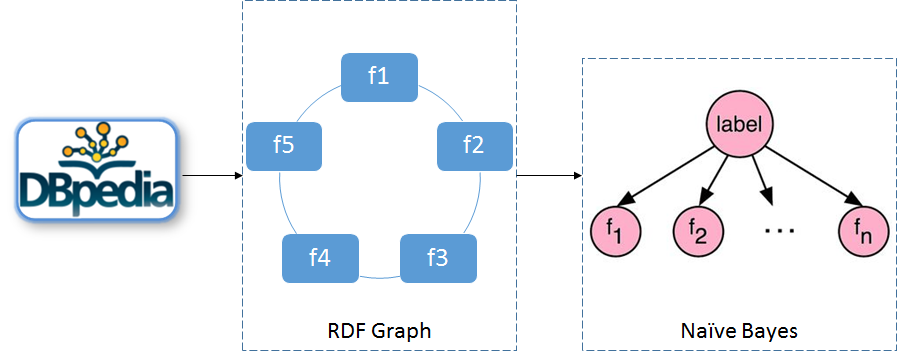
\includegraphics[width=\textwidth]{workflow.png}
	\caption{Sample workflow for \textit{Naive Bayes}}
	\label{nb}
\end{figure}

\textit{Naive Bayes} is a probabilistic classifier which applies the bayes theorem. \textit{Naive Bayes} constructs a joint probability table of all the attributes, it is using for the purpose of classification. The method makes the assumption that there is conditional independence between variables. The workflow in the figure above [\ref{nb}]  shows a sample workflow using the method and a knowledge base. Consider a data set which contains the variables \textit{f1...fn}. A knowledge base (such as DBpedia) can be searched for attributes \textit{f1..fn}, to get a connected graph showed how the attributes are linked and connected. This interlinking is used to inform \textit{Naive Bayes} that variables \textit{f1} and \textit{f2} may not be conditionally independent. This can be used to create a joint variable.
Also, the knowledge base graph provides other information such as the degree to which the two attributes (entities) are linked and how they linked. The attribute in the training set, can be combined with the data to give us a set of derived attributes which can be additionally used in the method.

\section{Updating the knowledge base}
As the knowledge base helps to improve the classifier, the test data can be used to update the links between entities in the knowledge base. The test data can be used to update missing values in the knowledge base of the attributes used in the statistical model. This raises important questions such as the data provenance as it may corrupt the knowledge base. The other option is to use Probabilistic Latent Semantic Analysis (PLSA) \cite{hofmann1999probabilistic} to find correlated variables in the training / test data.

\section{The Larger Picture}
\begin{figure}[h]
	\centering
	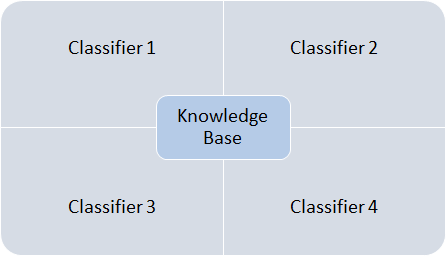
\includegraphics[width=7cm,height=4cm]{big_picture.png}
	\caption{\textit{The Mind Framework}}
	\label{lp}
\end{figure}

The above diagram [\ref{lp}] shows the larger framework where the knowledge base is used a passive entity by a multiple of classifiers. The framework tries to accomplish the following:
\begin{enumerate}
\item A method by which a classifier can use a knowledge base to understand the semantics of the data set and improve classification accuracy.
\item Use the test data set to improve the interlinking between entities in the knowledge base.
\item A knowledge base acts as a intermediate for classifiers to interact with each other.
\end{enumerate}

\bibliography{ref}{}
\bibliographystyle{plain}

\end{document}